%*******************************************************************************
%*********************************** First Chapter *****************************
%*******************************************************************************

\chapter{Grundlagen}  %Title of the First Chapter

\ifpdf
    \graphicspath{{Figs/Raster/}{Figs/PDF/}{Figs/}}
\else
    \graphicspath{{Figs/Vector/}{Figs/}}
\fi


%********************************** %First Section  **************************************

\section{Definition}
Ein Computer Emergency Response Team (CERT) (Deutsch: ```Computer-Notfall-Team```) ist ein Team, welches sich um IT-Sicherheit kümmert. Es analysiert mögliche Bedrohungen und wirkt möglichen Angriffen und Bedrohungen bereits vor dem Eintreten entgegen. Sollte es trotzdem zu einem Angriff kommen, ist das CERT verantwortlich die Ursachen zu ermitteln, dagegen vorzugehen und unterstützt bei der Wiederaufnahme des Regelbetriebs massgeblich mit.

\section{CERT und CSIRT}
\paragraph{CERT}Der Begriff ``CERT`` wurde vom Software Engineering Institute an der Carnegie Mellon University geprägt. Die CERT Devision arbeitet u.a. an der Forschung von Cybersecurity-Themen. Der Fokus liegt hierbei jedoch nicht nur auf der Forschung, sondern auch an der Entwicklung von Informationen zu IT-Sicherheitsthemen. Zusätzlich arbeitet die Devision auch mit Softwareherstellern, um die Sicherheit von Softwareprodukten zu erhöhen.~\citep{cert} Die CERT Devision wurde im Jahre 1988 nach dem Auftreten des Morris-Wurms an der Carnegie Mellon University in Pittsburg, Pensylvania in den USA gegründet.~\citep{homonym} Finanziert wurde diese Gründung durch das amerikanische Department of Defense. In den USA ist der Begriff ```CERT``` markenrechtlich geschützt und gehört der Carnegie Mellon University.
\paragraph{CSIRT}Aus diesem Grund werden CERT auch häufig als Computer Security Incident Responsive Team (CSIRT) bezeichnet. Es gibt jedoch auch einige Ausnahmen, wie z.B. der CERT-Bund des deutschen Bundesamtes für Sicherheit in der Informationstechnik. \\
\\
In dieser Arbeit werde ich beide Begriffe verwenden, wobei ich CERT als Markenname und CSIRT als Konzeptbegriff verwende.

\section{Grundlegende Aufgaben}
Durch das schnelle Wachstum und die Popularität des Internets befinden sich viele Firmen sehr schnell im Visier von Cyberattacken. Fast alle Firmen haben schützenswerte Informationen in ihren Systemen, welche deshalb genügend geschützt werden müssen. Bedrohungen sind nicht zwingend nur E-Spionage oder Konkurrenz. Bedrohungen durch das Internet reichen von ``normalen`` Viren und Ransomware~\citep{ransomware} bis zum gezielten Eindringen in Computernetzwerke von Firmen, um Daten zu entwenden oder zerstören. Eine komplette Abschottung und Eliminierung aller Angriffsvektoren ist Utopie, daher muss hierfür ein Mittelweg gefunden werden. \\
\\
Um diese Grundlage als CSIRT zu erfüllen, gehören folgende Aufgabenbereiche zum Tätigkeitsbereich eines CSIRTs:

\begin{itemize}
\item Analyse der Bedrohungslage
\item Erkennung von Angriffen im Voraus
\item Erkennung von momentanen Angriffen
\item Elimierung von momentanen Angriffen
\item Erarbeitung eines Notfallkonzeptes
\item Sofortiges Eingreifen in einer Bedrohungslage und direkte Massnahmen zur Sicherung und Notfall-Betriebes von kritischen Geschäftsprozessen
\item Unterstützung bei der Wiederaufnahme des Regelbetriebs
\item Koordination mit anderen CSIRTs
\end{itemize}

\section{Forum of Incident Response and Security Teams}
Nachdem 1988 das erste CERT an der Cornegie Mellon University gegründet wurde, gründete sich 1990 der Dachverband ``Forum of Incident Response and Security Teams``. \\
\\
Die FIRST fördert die globale Zusammenarbeit zwischen Notfallteams und definiert ``Best Practices``. Zudem werden Frameworks durch die FIRST zur Verfügung gestellt, welche den Aufbau und Betrieb von CERTs definieren, sowie auch Weiterbildungsmaterial um die globale Akzeptanz und das Wissen zu Security Incident Management zu fördern.

\section{CERT in der Schweiz}
Das bekannteste CERT in der Schweiz wird von SWITCH Information Technology Services gestellt. SWITCH ist verantwortlich für die .ch und .li Domains. Zusätzlich erbringt SWITCH auch Dienstleistungen im nationalen Forschung- und Bildungsnetzwerk und verlinkt Schweizer Universitäten mit anderen, internationalen Universitäten.\\
\\
Dank des CERTs der SWITCH ist die Schweizer Top Level Domain (TLD) eine der sichersten der Welt und die sicherste TLD Europas. ~\citep{switch}

\subsection{Gründung des SWITCH CERT}
Die CERT-Abteilung von SWITCH existiert bereits seit 20 Jahren. 1994 wird der Aufbau einer Fachstelle für Sicherheitsfragen geschaffen. Gemäss Geschäftsbericht der SWITCH dieses Jahres werden bereits einige sicherheitsrelevante Anfragen von Kunden der SWITCH beantwortet und die SWITCH informierte über bekanntgewordene Sicherheitsverletzungen. Die Akkreditierung der SWITCH-CERT erfolgt 1996 durch das CERT/CC der CERT-Koordinationsstelle der Carnegie Mellon University.

\section{CERT in Deutschland}
Auch in Deutschland sind mehrere CERTs tätig. Neben dem CERT der Universität Stuttgart sowie dem CERT des deutschen Forschungsnetzwerkes hatte sich auch Mcert etabliert. Das Mcert richtete sich vorallem an kleine und mittlere Unternehmen. Mittlerweile existiert die Mcert nicht mehr und wird durch das neu erschaffene CERT-Bund weitergeführt.

\subsection{CERT-Bund}

CERT-Bund ist die CERT des  Bundesamts für Sicherheit in der Informationstechnik (BSI). \\
\\
``CERT-Bund hat das Ziel als zentrale Anlaufstelle für präventive und reaktive Maßnahmen mit Bezug auf sicherheits- und verfügbarkeitsrelevante Vorfälle in Computersystemen zu fungieren. IT-Sicherheitsvorfälle werden in Zusammenarbeit mit Betroffenen von CERT-Bund bearbeitet.``~\citep{certbund} \\
\\
Das CERT-Bund bietet unter anderem folgende Dienstleistungen an: 24-Stunden-Support, Betrieb eines Lagezentrums, Analyze von und Empfehlungen zu Vorfällen anhand von Meldungen, Warndienste, Alarmierung der Bundesverwaltung

\subsection{Bürger-CERT}
Da das CERT-Bund nicht alle Anliegen von Privaten bearbeiten kann, wurde eine separate CERT ins Leben gerufen. Dieses Projekt untersteht auch dem deutschen BSI. Privatpersonen sowie Unternehmen können sich kostenlos diverse Dienstleistungen wie z.B. Gefährdungsnewsletter und -Alarmierungen via E-Mail abonnieren. So können sich auch kleinere Unternehmen über die Gefahrenlage informieren und proaktiv nach der Alarmierung gegen Gefahren schützen.

\section{Security Incident Management}
Security Incident Management bezeichnet das Vorgehen, wie bei Bedrohungen der IT-Sicherheit vorgegangen werden muss. Dies involviert Monitoring und Erkennen von Bedrohungen in Computer oder Computer-Netzwerken. Tritt ein Incident (Event) ein, wird dieses gemäss definiertem Prozess effektiv behandelt. Wie ein solcher Prozess aussehen kann, wird später veranschaulicht. \\
\\
Security Incident Management ist die Grundlage für CISRT. Ohne Definition, wie mit Security Incidents umgegangen werden soll, kann das Response Team nicht arbeiten. Security Incident Management ist eines der wichtigsten Teilgebiete der IT-Security und dadurch Teil der ISO-27000 Familie. ISO-27035~\citep{iso27035} definiert die Grundlagen für das Security Incident Management und definiert fünf Phasen.

\subsection{Phase 1: Prepare}
In der Vorbereitungsphase ist das Ziel ein CSIRT aufzubauen und die dafür benötigten Prozessgrundlagen zu erarbeiten. Sobald diese Prozesse und das Team definiert sind, kann mit dem Monitoring von Bedrohungen und Identifizieren von Incidents fortgeführt werden. \\
\\
Wichtige Fragen:
\begin{itemize}
\item Wie soll auf ein Incident reagiert werden?
\item Wer reagiert wie und wann?
\item Wie ist der Eskalationsprozess aufgebaut?
\item Wie setzt sich das Response Team zusammen?
\item Wer wird wann informiert?
\item Wo werden Incidents dokumentiert?
\item Wie werden Incidents in Zukunft vermieden?
\end{itemize}

\subsection{Phase 2: Identify}
In der Identifikationsphase geht es darum, dass Bedrohungen und Incidents schnell und korrekt identifiziert werden können. Sobald ein Incident identifiziert wird, muss dieser sofort gemäss Prozessdefinition gemeldet werden. Je nach Prozess kann dies in verschiedenen Tools gemeldet werden. Ein Beispiel dafür wäre ein Ticket beim Service Desk. Hierbei ist es wichtig, dass die korrekte Prioriät übernommen wird und nicht innerhalb der anderen Tickets untergeht.\\
\\
Der ISO-27035-Standard definiert Vorlagen für das Reporting von Security Incidents. Diese dürfen entsprechend verwendet werden und können, falls nötig, auch an die eigene Unternehmensstruktur angepasst werden.

\subsection{Phase 3: Assess}
In der Assess-Phase wird ermittelt, wie mit diesem Incident vorgangen werden kann.\\
\\
Fragen, die sich das CSIRT stellen muss in dieser Phase beinhalten unter anderem:

\begin{itemize}
\item Muss das System offline genommen werden bis der Incident behoben ist?
\item Müssen forensische Daten gesammelt werden, bevor das System wieder funktionstüchtig gemacht werden kann?
\item Reicht es aus, das System zu patchen und wieder online zu bringen?
\item Muss das System komplett neu aufgesetzt werden?
\end{itemize}

\subsection{Phase 4: Respond}
Sind die möglichen Optionen klar und die beste(n) davon gewählt, muss der Incident behoben werden. Die definierten Aktionen werden durchgeführt bis das System wieder im Normalbetrieb ist. Ist dies erledigt, kann der Incident geschlossen werden.

\subsection{Phase 5: Learn}
Der Incident ist zwar gelöst, aber der Prozess ist noch nicht fertig angewendet. Phase 5 definiert ``Lessions learnt``. Um in der Zukunft besser und effektiver auf einen Incident zu reagieren, werden die durch diesen Incident gewonnenen Erkenntnisse analysiert und dokumentiert. Nur so kann sichergestellt werden, dass sich das CSIRT mit den Erkenntnissen auseinandersetzt und diese dazu verwendet, den Prozess zu optimieren. Da ein Prozess nie perfekt ist, sollten diese Erkenntnisse in die Prozessoptimierung einfliessen. Dabei ist es wichtig, dass dies regelmässig gemacht wird, damit der Prozess immer möglichst effektiv und effizient abgearbeitet werden kann.

\begin{figure}
  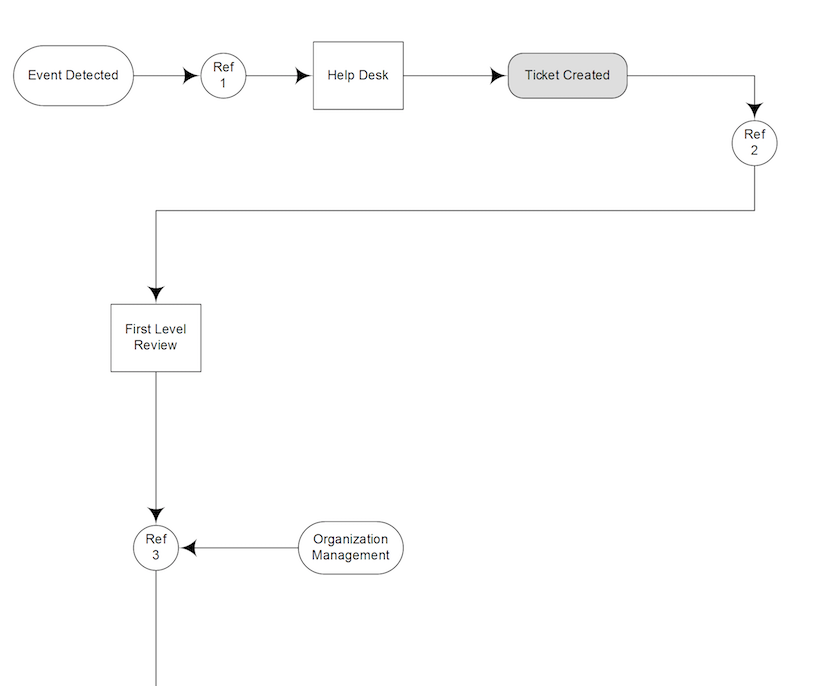
\includegraphics[width=\textwidth]{SIMExample}
    \caption{Auszug aus einem Security Incident Management Workflow. Image: CC-BY 2.5, Autor: Michael Berman}
    \label{fig:SIMExample}          
\end{figure}

\nomenclature[z-cert]{$CERT$}{Computer Emergency Response Team}
\nomenclature[z-csirt]{$CSIRT$}{Computer Security Incident Response Team}
\nomenclature[z-tld]{$TLD$}{Top Level Domain}
